\documentclass{beamer}
\usetheme[pageofpages=of,% String used between the current page and the
                         % total page count.
          bullet=circle,% Use circles instead of squares for bullets.
          titleline=true,% Show a line below the frame title.
          alternativetitlepage=true,% Use the fancy title page.
       %   titlepagelogo=logo-polito,% Logo for the first page.
       %   watermark=watermark-polito,% Watermark used in every page.
       %   watermarkheight=100px,% Height of the watermark.
       %   watermarkheightmult=4,% The watermark image is 4 times bigger
                                % than watermarkheight.
          ]{Torino}

\setbeamertemplate{footline}{
  \begin{beamercolorbox}[wd=\paperwidth,ht=1ex,dp=1ex]{footline}
    \vspace{5pt} \hspace{1em} \insertframenumber/\inserttotalframenumber
  \end{beamercolorbox}
}

\author{Brendon J. Brewer}
\title{STATS 331 -- Introduction to Bayesian Statistics}
\institute{The University of Auckland}
\date{}


\linespread{1.3}
\usepackage{minted}
\usepackage[utf8]{inputenc}
\usepackage{dsfont}
\newcommand{\given}{\,|\,}
\newcommand{\balpha}{\boldsymbol{\alpha}}
\newcommand{\bmu}{\boldsymbol{\mu}}


\begin{document}

\frame{\titlepage}

\begin{frame}
\begin{center}
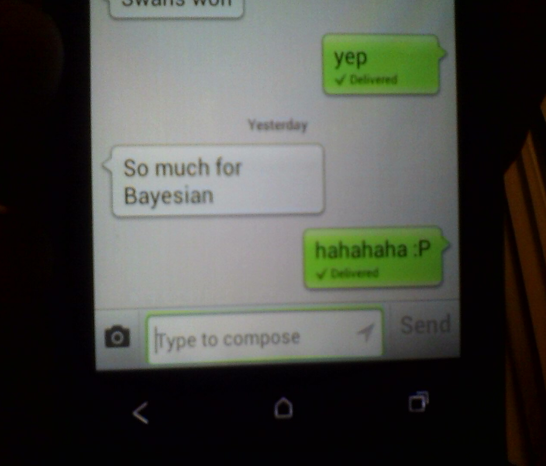
\includegraphics[width=0.7\textwidth]{images/dad.png}
\end{center}

\end{frame}


\begin{frame}
\centering
\Large
Two unrelated subjects:
One-way ANOVA and Posterior Predictive Checks

\end{frame}


\begin{frame}
\frametitle{Reminder of T-Tests}

\begin{center}
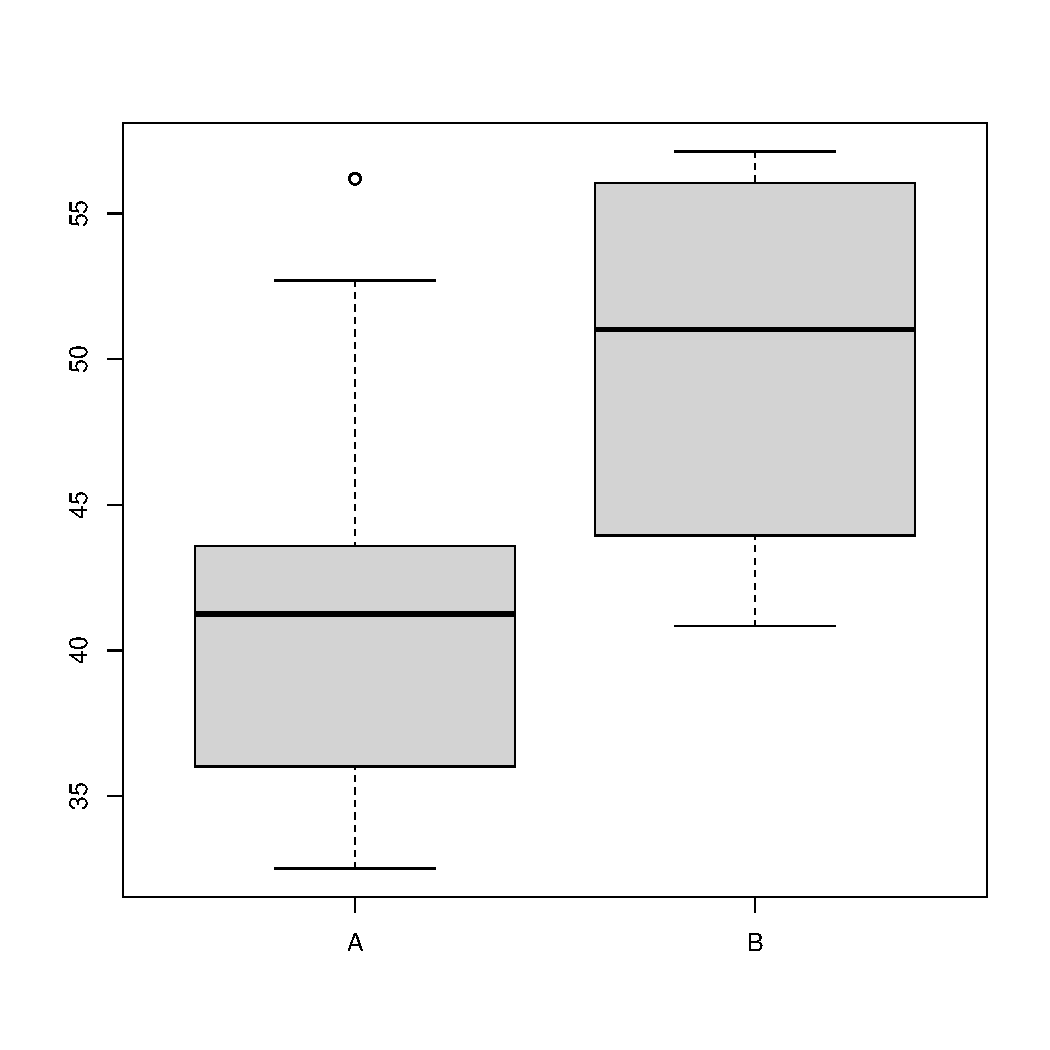
\includegraphics[width=0.6\textwidth]{images/widgets_boxplot.pdf}
\end{center}

\end{frame}

\begin{frame}[fragile]
\frametitle{Reminder of T-Test Model 3}
Recall T-Test Model 3, which modelled the idea that the group mean
parameters $\mu_1$ and $\mu_2$ might be close together or far apart, but not
exactly equal. The priors were hierarchical:\pause
\footnotesize

\begin{minted}{r}
grand_mean ~ dnorm(0, 1/1000^2)
log_diversity ~ dunif(-10, 10)
diversity <- exp(log_diversity)
mu1 ~ dnorm(grand_mean, 1/diversity^2)
mu2 ~ dnorm(grand_mean, 1/diversity^2)
log_sigma ~ dunif(-10, 10)
sigma <- exp(log_sigma)
\end{minted}

\end{frame}


\begin{frame}[fragile]
\frametitle{Reminder of T-Test Model 3}
(Zoomed in)
\begin{center}
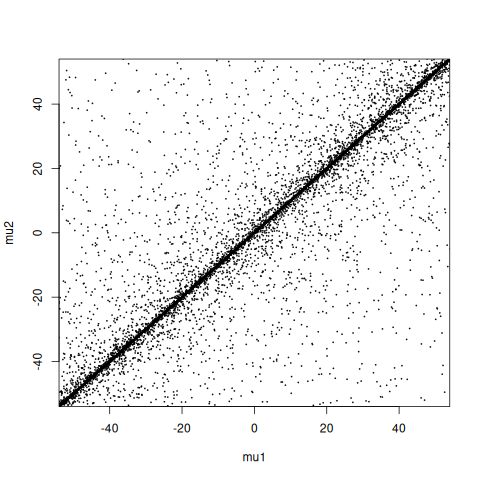
\includegraphics[width=0.5\textwidth]{images/ttest_prior3.png}
\end{center}

\end{frame}



\begin{frame}[fragile]
\frametitle{Reminder of T-Test Model 3}
The sampling distribution/likelihood part of T-Test Model 3 was very
formulaic:

\begin{minted}{r}
for(i in 1:N1)
{
    x1[i] ~ dnorm(mu1, 1/sigma^2)
}
for(i in 1:N2)
{
    x2[i] ~ dnorm(mu2, 1/sigma^2)
}
\end{minted}

\end{frame}



\begin{frame}[fragile]
\frametitle{Example Data: More Groups}

\begin{columns} % Create two columns
    \column{0.4\textwidth} % Left column (50% width)
    \begin{itemize}
    \item Masses of starlings, in grams, at four different locations.
    \item The locations don't have an order to them, so we are not doing
          simple linear regression.
    \end{itemize}

    \column{0.6\textwidth} % Right column (50% width)
    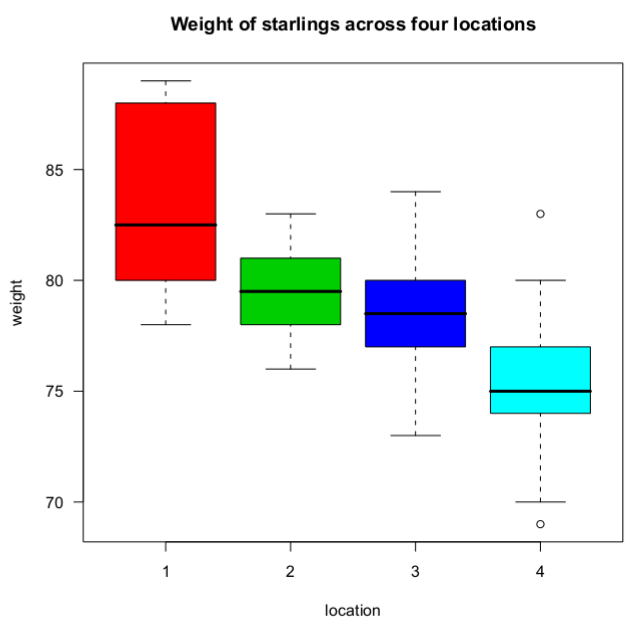
\includegraphics[width=1\linewidth]{images/starling.png}
 \end{columns}


\end{frame}

\begin{frame}[fragile]
\frametitle{One-way ANOVA}
In classical statistics, we might be interested in the hypothesis
\begin{align}
H_0:\quad \mu_1 = \mu_2 = \mu_3 = \mu_4.
\end{align}
\pause

The method for handling this classically is one-way analysis of variance
(ANOVA). We will instead make a Bayesian model that is similar to T-Test
Model 3, but for more groups. We give up on a precise $H_0$.
We also don't analyse any variance!

\end{frame}



\begin{frame}[fragile]
\frametitle{Starling Data: CSV File}
The data is in a different format compared to before (all masses are in one
vector).
\begin{minted}{r}
"location","Y"
1,78
1,88
1,87
...
2,78
2,78
2,83
...
\end{minted}

\end{frame}


\begin{frame}[fragile]
\frametitle{One-way ANOVA: Sampling Distribution}
Because of the new data format, we need to rewrite the JAGS
code for the sampling distribution/likelihood.

\begin{minted}{r}
for(i in 1:length(Y))
{
    Y[i] ~ dnorm(mu[location[i]], 1/sigma^2)
}
\end{minted}
\pause
We now need priors for the four \mintinline{r}{mu} parameters
and also \mintinline{r}{sigma}.

\end{frame}


\begin{frame}[fragile]
\frametitle{One-way ANOVA: Priors}
The priors will be very similar to T-Test Model 3, except our
\mintinline{r}{mu} parameters are now in a vector.
\footnotesize
\begin{minted}{r}
grand_mean ~ dnorm(0, 1/1000^2)
log_diversity ~ dunif(-10, 10)
diversity <- exp(log_diversity)
for(i in 1:4)
{
    mu[i] ~ dnorm(grand_mean, 1/diversity^2)
}
log_sigma ~ dunif(-10, 10)
sigma <- exp(log_sigma)
\end{minted}

\end{frame}


\begin{frame}[fragile]
\frametitle{Running JAGS}
Let's run JAGS on the starling data and look at the following outputs:

\begin{itemize}
\item The trace plots for the \mintinline{r}{mu}s.\pause
\item The posterior probability that \mintinline{r}{mu[2] > mu[3]}.\pause
\item The posterior distribution for \mintinline{r}{log_diversity},
which describes the degree to which the $\mu$s are different from each other.
\end{itemize}


\end{frame}

\begin{frame}[fragile]{Shrinkage and Borrowing Strength}
Since the prior for the $\mu$ parameters is dependent, learning one
tells you about another. Similarly, learning {\em about} one from some data
provides information about the others.\pause

The posterior for
$\mu_1$ is narrower than you would get from analysing group 1's data alone.
Estimates of $\mu_1$ are also dragged a little bit towards the average mass
for the {\em other} groups.
\pause

To understand why this happens, imagine if all the {\em other} groups' data
told you the hyperparameters with no uncertainty. What would your
prior for $\mu_1$ become?
\end{frame}


\begin{frame}[fragile]
\frametitle{Pre-Whitening}

\begin{itemize}
\item Recall that, due to the way the hierarchical model is constructed,
the prior for the $\mu$ parameters is actually correlated.\pause
\item JAGS uses MCMC methods that perform worse when the {\em posterior}
is correlated.\pause
\item If the prior is correlated, that makes it more likely that the posterior
is also.\pause
\item ``Pre-whitening'' can sometimes help --- we will write the same prior
assumptions but in a way that makes the parameters' priors independent.
\end{itemize}


\end{frame}

\begin{frame}[fragile]
\frametitle{Pre-Whitening}
\begin{minted}{r}
for(i in 1:4) # Original form
{
    mu[i] ~ dnorm(grand_mean, 1/diversity^2)
}

for(i in 1:4) # Modified form, all priors independent
{
    n[i] ~ dnorm(0, 1)
    mu[i] <- grand_mean + diversity*n[i]
}
\end{minted}

\end{frame}


\begin{frame}[fragile]
\frametitle{Pre-Whitening}
In this example, the pre-whitening doesn't actually make much difference.
By the way, the term comes from {\bf white noise} which is noise where
every value is independent.
\end{frame}


\begin{frame}
\centering
\Large
Posterior Predictive Checks

\end{frame}


\begin{frame}
\frametitle{The Good News}
\begin{itemize}
\item Bayesian statistics always works...\pause
\item {\bf If} your prior beliefs are well described by the prior,
and your knowledge of how the data and parameters are related is well described
by the sampling distribution.\pause
\item Also you need to be able to do the calculations :-)
\end{itemize}


\end{frame}


\begin{frame}
\frametitle{The Bad News}
\begin{itemize}
\item For silly choices of prior and/or likelihood, it is possible to get
a silly posterior distribution. It is not always obvious that a particular choice
is silly (in a way that matters).\pause
\item In practice, choices are often based on convenience and tradition.
\end{itemize}


\end{frame}


\begin{frame}
\frametitle{Spherical Cow in a Vacuum}
\url{https://en.wikipedia.org/wiki/Spherical_cow}

\begin{center}
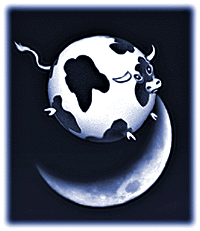
\includegraphics[width=0.4\textwidth]{images/spherical_cow.png}

Credit: Ingrid Kallick (\url{http://www.ikallick.com/})
\end{center}


\end{frame}



\begin{frame}
\frametitle{Simple Linear Regression Example}
We will use a simple linear regression example to illustrate the idea
of {\bf posterior predictive checks}, which are used to get some insight into
the model assumptions being used.

\end{frame}


\begin{frame}
\frametitle{Simple Linear Regression: Fake Data}
I will generate some data from the curved relationship:
\begin{align}
y_i &= \beta_0 + \beta_1 x_i + \beta_2 x_i^2 + \epsilon_i\\
\epsilon_i &\sim \textnormal{Normal}(0, \sigma^2)
\end{align}

\pause

But we will fit the data without the quadratic term.


\end{frame}

\begin{frame}
\frametitle{Simple Linear Regression: Fake Data}
\begin{minted}{r}
set.seed(123)
x = seq(-3, 3, length=100)
y = 1 + x + x^2 + rnorm(length(x))

data = data.frame(x=x, y=y)
write.csv(data, "quadratic_data.csv", row.names=FALSE)
\end{minted}

\end{frame}

\end{document}

